\lhead{\emph{\ChapterThree{}}}
\label{classification-conclusions}
El primer acercamiento de clasificación se realizó utilizando los metadatos disponibles para cada uno de los TFGs, concretamente el título y el abstracto. Se utilizó el campo de "tema" para determinar la clasificación que se le había dado a cada TFG en el RIULL.
%

Se realizó una batería de pruebas, variando el número de palabras comunes a considerar. Se empezó utilizando las 100 palabras más comunes, aumentando esto en incrementos de 100 hasta llegar a un clasificador que considera las 2000 palabras más comunes entre los textos a clasificar.

\begin{center}
\begin{figure}[!ht]
  \label{fig:metadata_view}
  \centering
    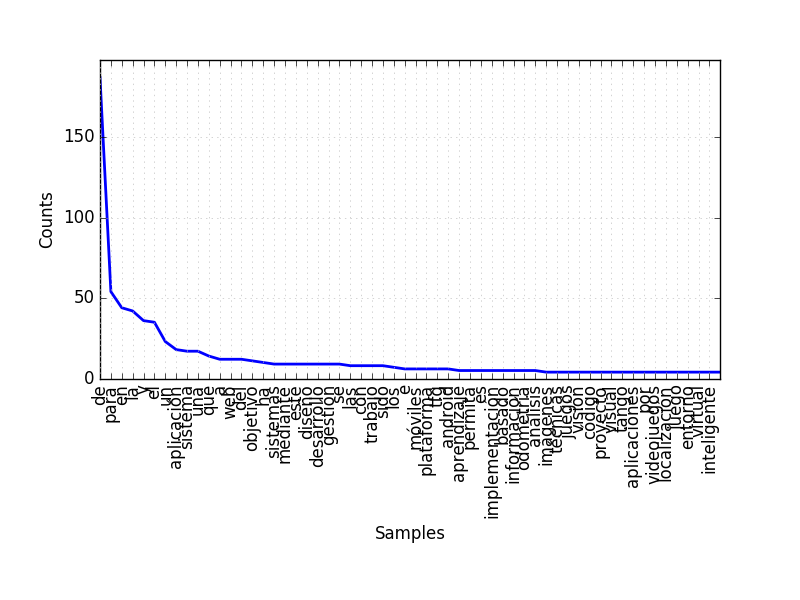
\includegraphics[width=0.8\textwidth]{Images/clas1-words}
  \caption{Palabras de mayor frecuencia entre las instancias de la primera aproximación.}
\end{figure}
\end{center}

Se tiene aquí un histograma de las palabras de mayor frecuencia entre las instancias de la primera aproximación del caso de estudio, que se corresponden con los metadatos de los TFG del Grado en Ingeniería Informática.
%
Como se puede apreciar, la información es muy pobre, dado que las palabras más comunes son preposiciones, encabezadas por \texttt{de}, que aparece 187 veces. La palabra \texttt{aplicación} es la primera palabra significativa y aparece 18 veces, seguida de \texttt{sistema} con 17 apariciones.
%
Las palabras relevantes se repiten muy pocas veces en el corpus creado, con lo cual es difícil realizar inferencias en bases a ellas.

\begin{center}
\begin{figure}[!ht]
  \label{fig:metadata_view}
  \centering
    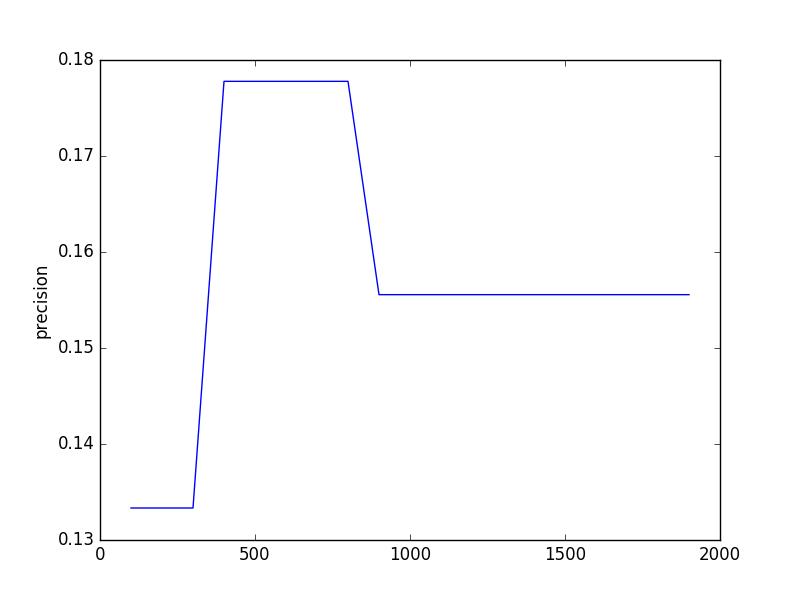
\includegraphics[width=0.8\textwidth]{Images/clas1-precision}
  \caption{Precisión de la clasificación Naive Bayes usando metadatos de los TFG de Ing. Informática.}
\end{figure}
\end{center}

Como vemos, la precisión del clasificador oscila entre 0.13 y 0.18, lo que indica que el clasificador acierta entre el 13\% y 18\% de las veces. Estos resultados son bastante pobres, y esto se debe a la poca información que proporcionan los metadatos existentes sobre los textos.
%
La falta de información se debe a tres factores: en primer lugar, los títulos no suelen sobrepasar las 20 palabras, lo que hace difícil la clasificación por conteo de palabras comunes. 
%
El segundo problema es que en muchos casos, la descripción o abstracto del TFG no se encuentra como metadato del TFG en el
RIULL, debido a ser un campo opcional.
%
Finalmente, se tiene un número elevado de clases, muchas de ellas conteniendo a un único TFG, lo que reduce las posibilidades de caracterizar una clase y aumenta las probabilidades de cometer una asignación errónea.

Por otra parte, podemos observar cómo decrementa la precisión del clasificador a partir de un número de palabras dado. Podemos inducir de esto que existe un límite de palabras a considerar óptimo, tras el cual se consideran demasiadas características de los elementos como para dar una respuesta fiable.

\vskip 20px

El segundo acercamiento realizado consistió en la obtención de los metadatos de todos los Trabajos de Fin de Grado en el RIULL.
Esto resultó en un incremento considerable de la cantidad de instancias, pasando de los 91 TFG de Ing. Informática a 350 documentos.
%
Al igual que en el caso más reducido de los TFG de Ing. Informática, la gran mayoría de los Trabajos de Fin de Grado no contienen un abstracto como metadato, provocando que nos limitemos a utilizar únicamente sus títulos en su mayor parte.

\begin{center}
\begin{figure}[!ht]
  \label{fig:metadata_view}
  \centering
    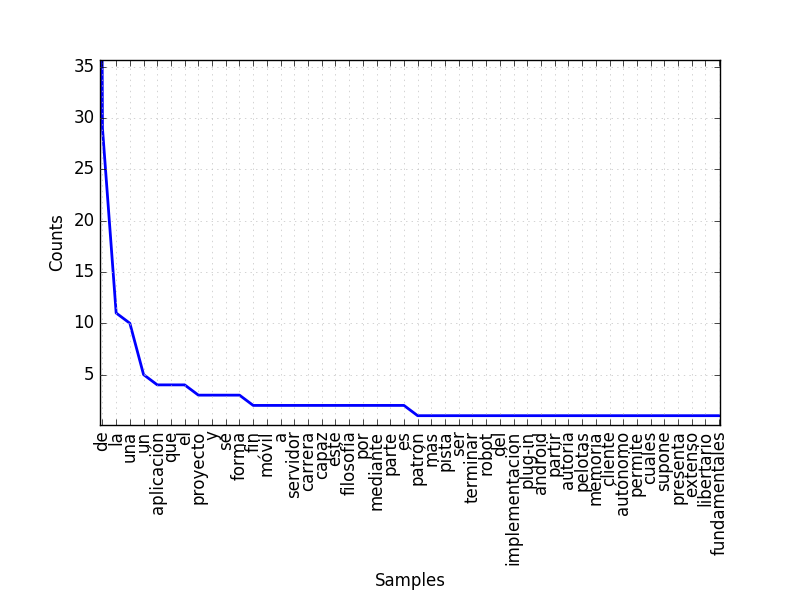
\includegraphics[width=0.8\textwidth]{Images/clas2-words}
  \caption{Palabras de mayor frecuencia entre las instancias de la segunda aproximación.}
\end{figure}
\end{center}

\begin{center}
\begin{figure}[!ht]
  \label{fig:metadata_view}
  \centering
    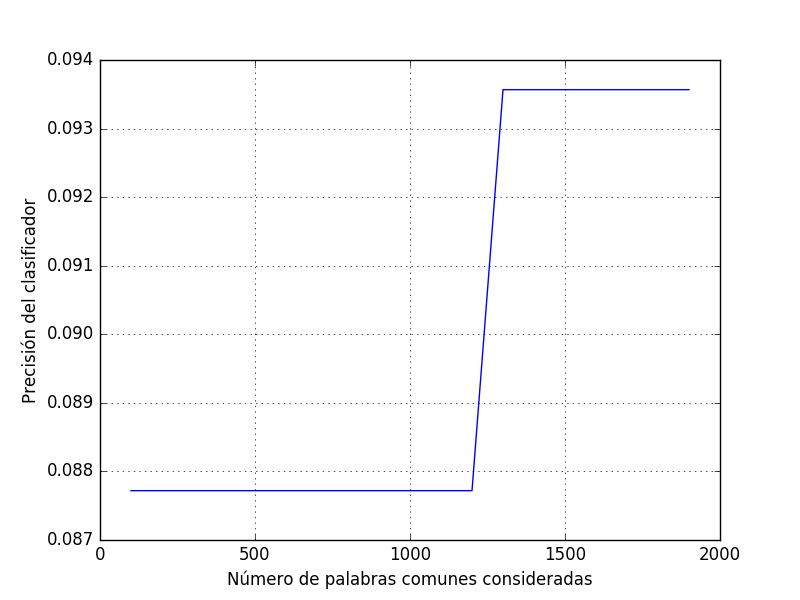
\includegraphics[width=0.8\textwidth]{Images/clas2-precision}
  \caption{Precisión de la clasificación Naive Bayes usando metadatos de todos los TFG del RIULL.}
\end{figure}
\end{center}

Como podemos apreciar, el leve incremento en la cantidad de datos disponibles no evita que esta aproximación tenga menos éxito que la anterior en base al subproblema escogido.  Mientras el primer clasificador oscilaba entre el 13\% y 18\% de acierto, éste clasificador se mueve entre el 8\% y 10\% de efectividad.
%
Este clasificador tiene una menor eficacia que el del anterior caso, pero hay que tener en cuenta que hace frente a un problema de mayor dificultad: en la aproximación anterior tratábamos con 14 clases, mientras que en éste caso se dan 28 clases distintas.